%
\documentclass[%
 reprint,
 amsmath,amssymb,
 aps,
]{revtex4-1}

\usepackage{graphicx}% Include figure files
\usepackage{dcolumn}% Align table columns on decimal point
\usepackage{bm}% bold math


\begin{document}


\title{INMON VS  KIMBALL}
\author{Panty Sihuayro, Juan Carlos          }
\author{Huilca Umpiri ,William Arturo 	  }
\author{Esperilla Ruiz , Adnner Sleyder 	  }

		
\affiliation{%
 Universidad Privada de Tacna \textbackslash Facultad de Ingenieria \textbackslash Escuela Profesional de Ingenieria de Sistemas
}%

\begin{abstract}
\begin{center}
\textbf{Resumen}
\end{center}
Los almacenes de datos (data warehouses en inglés) toman cada día mayor importancia, a medida que las organizaciones pasan de esquemas de sólo recolección de datos a esquemas de análisis de los mismos. En este breve artículo se  tratará de brindar una explicación general de algunas metodologías, en este caso serán la metodología Kimball y la metodología Inmon.
\\

\begin{center}
\textbf{Abstract}
\end{center}
Data warehouses (data warehouses in English) are becoming increasingly important, as organizations move from data-only schemes to data analysis schemes. In this short article we will try to provide a general explanation of some methodologies, in this case they will be the Kimball methodology and the Inmon methodology.
\\
\end{abstract}



\maketitle

%\tableofcontents

\section {Introducción}\label{sec:1}

Estamos viviendo en la era de una revolución de datos, y más corporaciones se están dando cuenta de que para liderar, o en algunos casos, para sobrevivir, necesitan aprovechar su riqueza de datos de manera efectiva. El almacén de datos, debido a su propuesta única como repositorio empresarial integrado de datos, está jugando un papel aún más importante en esta situación. Actualmente se practican dos estilos de arquitectura prominentes para construir un almacén de datos: la arquitectura Inmon y la arquitectura Kimball. Este documento intenta comparar y contrastar los pros y los contras de cada estilo de arquitectura y recomendar qué estilo seguir basándose en ciertos factores.\cite

%-----------------------------------------------------------------
\section{Objetivos}\label{sec:2}
\subsection{General:}
Dar una visión clara de BI, desde las perspectivas de los autores que sentaron las bases que son Ralph Kimball y Bill Inmon, para la mejora de las estrategias del negocio al que se desee implementar las herramientas de BI.
\subsection{Específicos:}
 Describir las metodologías propuestas por los principales autores de BI desde las perspectivas de sus creadores Ralph Kimball y Bill Inmon.
 
 
 

%-----------------------------------------------------------------
\section {Marco Teórico}

\subsection{METODOLOGIA SEGUN INMON}	
Según Bill Inmon, propone que un DW es el conjunto de datos orientados a temas específicos de la organizaciones, es decir deberán ir cambiando con el transcurso del tiempo, pero dichos datos, no deben ser volátiles (no es posible eliminar, ni modificar la información).
Al momento de generar un cambio en los datos, se debe de efectuar de una manera que, quede reflejado el cambio que se efectuó y mantener siempre la integridad de la información, se espera que todo resultado del proceso y transformación de la información por medio de herramientas de BI, sea un firme apoyo para los tomadores de decisiones al momento de orientar una estrategia de negocio.
. \cite



Consta de las siguientes características:
\begin{itemize}
		\item \textbf{Orientado a temas:} Los datos en la base de datos están organizados de manera que todos los elementos de datos relativos al mismo evento u objeto del mundo real queden unidos entre sí.
		\item \textbf{Integrado:} La base de datos contiene los datos de todos los sistemas operacionales de la organización, y dichos datos deben ser consistentes. 
		
		\item \textbf{No volátil:} La información no se modifica ni se elimina, una vez almacenado un dato, éste se convierte en información de sólo lectura, y se 	mantiene para futuras consultas.
		\item \textbf{Variante en el tiempo:}Los cambios producidos en los datos a lo largo del tiempo quedan registrados para que los informes que se puedan generar reflejen esas variaciones.

	\begin{center}
					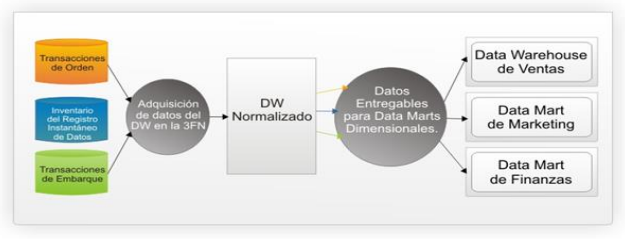
\includegraphics[width=9cm]{./IMAGENES/imgleydi2}
				\end{center}
\end{itemize}




\subsection{ARQUITECTURA SEGUN INMON}
\begin{figure}[htb]
			
			\end{figure}

La arquitectura que plantea Bill Inmon consta de las siguientes partes: \cite{aquino1}
\begin{itemize}
		\item Fuente de la Información: Inicia el proceso de creación de un DW, conociendo la información que se necesita de todas las herramientas de las que se tengan acceso, ir a las necesidades de información que se necesitan con la finalidad de un resultado para crear un DW.

		\item Data Warehouse: La necesidad de normalizar toda la información extraída para ser almacenada en un DW, los cuales serán procesados y consultados por un DM.
		\item Data Marts: Se crean un subconjunto de los datos de un DW con el objetivo de responder a un determinado análisis o necesidad de una población, de un departamento en específico.
		\item Explotación de los datos: Se refiere a la manera de presentación de la información para ser consultada y analizada por las áreas. En cuanto a la arquitectura interna de un DW, Bill Inmon considera las siguientes características:

			\begin{itemize}
				\item Normalización: el DW debe ser basado y diseñado, conforme al diseño de las bases de datos transaccionales con las que se esté interactuando.
				\item Tercera Forma normal: la prioridad es que el modelo de datos esté construido en TFN con lo cual se tenga mayor relación entre los objetos de la base de datos.
			\end{itemize}
			
			
			\begin{center}
					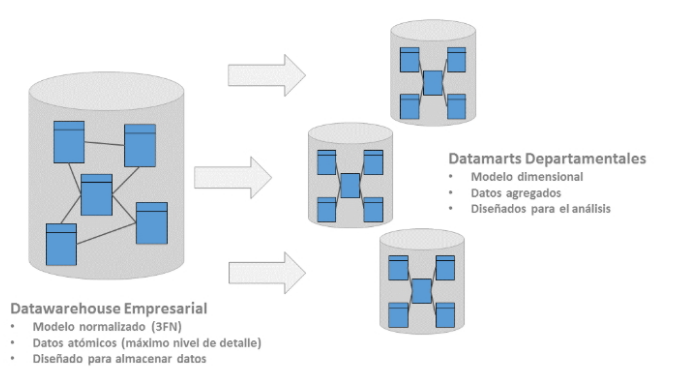
\includegraphics[width=9cm]{./IMAGENES/1}
				\end{center}

\end{itemize}





\subsection{METODOLOGIA SEGUN KIMBALL}	
En su metodología propuesta, menciona la relevancia de la información dentro de las
organizaciones y destaca dos propósitos principales: el primero hace referencia a que
el sistema operacional que realiza las transacciones de la organización, debe de ser
utilizado para el registro de la información y segundo, que los sistemas de DW/BI
deben ser utilizados para la consulta de los datos.
Según Ralph Kimball, promotor principal del enfoque dimensional define un Data
Warehouse como “una copia de los datos transaccionales específicamente para la
consulta y el análisis”(6), también parte de su metodología es la forma de construcción
del DW. A su vez define que un Data Mart es “Un repositorio de información similar a
un DW, pero orientado a una área o departamento”.
Propone algunas metas para la buena realización de los sistemas de Negocios
Inteligentes:


\begin{itemize}
	\item   Acceso a la información de manera rápida y fácil. 
	\item Credibilidad de la información, los datos deben pasar por un proceso de
depuración de la información, descartando la información innecesaria y no
relevante, verificación de la fuente de los datos.
 
	\item Adaptabilidad a través del tiempo, donde la Información debe estar
acompañada del Tiempo.
	\item Aplicación de controles de seguridad.
\end{itemize}

La construcción de una solución de DW/BI (Datawarehouse/Business Intelligence) es sumamente compleja, y Kimball nos propone una metodología que nos ayuda a simplificar esa complejidad. Las tareas de esta metodología (ciclo de vida) se muestranen la figura 1.

			


4.4.1. Arquitectura Ralph Kimball


				\begin{center}
					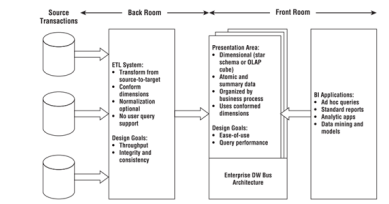
\includegraphics[width=9cm]{./IMAGENES/arqui}
				\end{center}
Para el desarrollo de su esquema los detalla en tres áreas.:

\begin{itemize}
	\item Source Transactions: En esta área está la base transaccional de la
organización, es decir la fuente de los datos.

	\itemBack Room: Es donde se encuentra el DW, para su llenado de información hace
uso de los sistemas ETL.

	\item FrontRoom: Conformado por el área de presentación y aplicaciones BI es la
parte final de la arquitectura donde se organiza y se logra visualizar la
información por parte de o de los usuarios finales.
 plan del proyecto.
\end{itemize}

ETL.
Extracción, transformación y cargado (en inglés extract, transformation, and load), está
en el área de back room, entre la fuente de datos y el área de presentación. La
extracción es la primera etapa la de obtención de los datos con el fin de leer, entender
y copiar los datos requeridos.  

4.4.2. Ciclo de vida

Gran parte de la metodología está basado en el ciclo de vida, el cual consta de 4
principios básicos:



\begin{itemize}
		\item Proyecto BI centralizado en el negocio: enfocar todos los esfuerzos a nivel
técnico y humano en desarrollar los requerimientos del proyecto con el negocio,
dar respuesta por medio de la investigación y el análisis de resultados.

		\item Diseñar una infraestructura de datos apropiada: Diseñar e implementar una
base de datos (o de información) única, de fácil uso y alto rendimiento, y este
integrada las plataformas de la organización.
		
		\item Realizar entregas: la carga de los datos en los DW debe ser gradual, dentro de
un plazo de 12 meses, esto está condicionado a los requerimientos del negocio.

		

	
\end{itemize}

%-------------------------------------------------
%-------------------------------------------------

\subsection{COMPARACION DE METODOLOGIAS}	
El datawarehouse de Kimball está orientado a la consulta de la información, por lo que su estructura interna está especialmente diseñada para garantizar una explotación de los datos rápida y sencilla, no requiriendo usuarios especializados para ello.\\
 Por el contrario, el datawarehouse de Inmon persigue la integración de todos los datos de la compañía, estando orientado hacia el almacenaje de grandes volúmenes de datos, por lo que su estructura interna normalizada se diseña para evitar la redundancia de datos, simplificar las labores de mantenimiento, etc.\citep{kumar}\\


				\begin{center}
					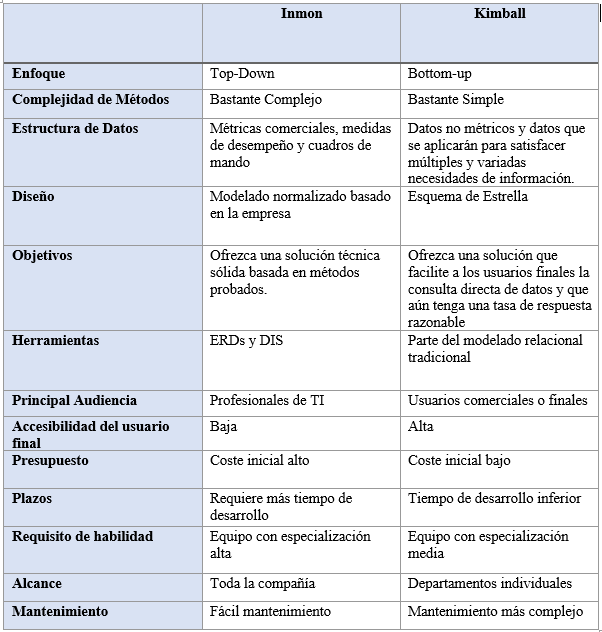
\includegraphics[width=9cm]{./IMAGENES/Inmon-Kimball}
				\end{center}


%-----------------------------------------------------------------
\section{Análisis}

\begin{itemize}
\item Podríamos decir que el enfoque de Kimball se ajusta mas a proyectos pequeños en los que se persiga un sistema fácilmente explotable y entendible por el usuario y de rapido desarrollo, siendo el modelo de Inmon mas apropiado para sistemas complejos de mayor envergadura.

\end{itemize}
%-----------------------------------------------------------------
\section{Conclusiones}

\begin{itemize}
\item La metodología de Kimball es ideal para los primeros pasos de implantación de BI a un cliente, cuando la complejidad de almacenamiento de datos no es demasiado grande y donde la infraestructura del BI se encarga de los datos procedentes de un número limitado de fuentes. Sin embargo, cuando el almacén de datos adquiere complejidad, entonces es peligroso forzar el desarrollo de esta metodología. En el mundo del BI, cuando las cosas adquieren gran complejidad, es el momento de introducir nuevos enfoques al problema, como el propuesto por Inmon.

\end{itemize}


% Bibliografia.
%-----------------------------------------------------------------

\bibliographystyle{plain}
\bibliography{Bibliografia}

\end{document}
